\chapter{Marco teórico}
Desarrollar métodos automáticos para analizar las acciones en videos es de particular importancia, primero se debe entender que acciones se dan en un video. El reconocimiento de acciones (patrones), que es el problema de asignar un video a un conjunto de clases de acción predefinidas, y la localización de acción, definida como la identificación de la localización spatio-temporal donde tiene lugar una acción, son dos de los temas fundamentales y muy estudiados en este contexto.

La mayoría de los marcos existentes para el reconocimiento de acciones consta de tres pasos principales: extracción de características, aprendizaje (entramiento de clases) para formar una representación de un video basado en las características extraídas y finalmente clasificación del video usando dicha representación.

En el primer paso, un conjunto de características, como STIP \cite{laptev2005space} o densa trayectorias \cite{wang2011action,
wang2013dense}, se extraen de un determinado video. Se supone que estas características codifican la información que es útil para el reconocimiento de la acción en una forma numérica (un vector). A continuación, las características extraídas se utilizan para formar una representación de un vídeo, que captura las acciones que se producen en el mismo. Tal representación puede ser tan simple como un histograma de los movimientos más frecuentes \cite{wang2011action,
wang2013dense} o un modelo semánticamente significativo. En el último paso, se aprende un modelo general para cada acción de interés usando la representación computarizada de un conjunto de vídeos de entrenamiento etiquetados.


\section{flujo óptico}
El flujo óptico es el patrón del movimiento aparente de los objetos de la imagen entre dos marcos consecutivos causados por el movimiento del objeto o de la cámara. Es un campo vectorial 2D donde cada vector es un vector de desplazamiento que muestra el movimiento de puntos desde el primer fotograma hasta el segundo. Considere la imagen de abajo (Imagen Cortesía: Artículo de Wikipedia sobre Flujo Óptico).

\subsection{Lucas-Kanadeen y flujo óptico}
OpenCV proporciona todo esto en una sola función, \textbf{cv2.calcOpticalFlowPyrLK ()}. El objetivos de esta técnica es crear una sencilla aplicacion para realizar un seguimiento a los puntos, usamos \textbf{cv2.goodFeaturesToTrack ()}. Tomamos el primer fotograma, detectamos algunos puntos de esquina de Shi-Tomasi (\ref{fig:datasetKth}) en él, entonces seguimos iterativamente esos puntos usando el flujo óptico de Lucas-Kanade. Para la función \textbf{cv2.calcOpticalFlowPyrLK ()} pasamos el fotograma anterior, los puntos anteriores y el fotograma siguiente. Devuelve los puntos siguientes junto con algunos números de estado que tiene un valor de 1 si se encuentra el siguiente punto, de lo contrario cero. Pasamos iterativamente los siguientes puntos como puntos anteriores en el siguiente paso. 
(figura \ref{fig:optical-flow1})

\begin{figure}[h!]

 % \centering
  \begin{subfigure}[]{0.4\linewidth}
      \centering 	  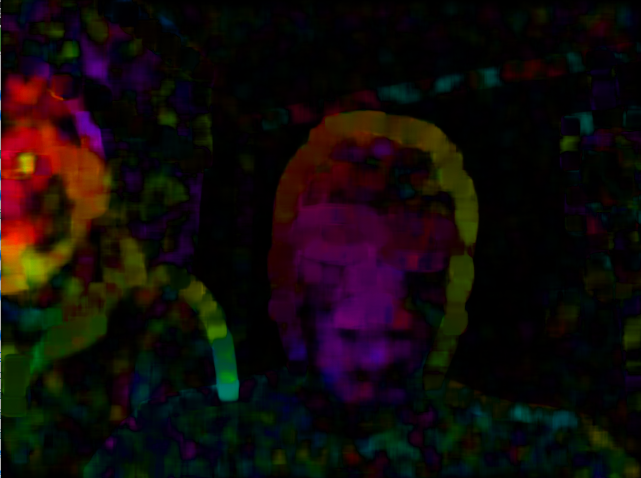
\includegraphics[width=0.4\textwidth]{Kap3/img/Dense_optical_flow_by_HSV_color_image.png}
  \caption{dense-optical-flow-HSV}     
  \label{fig:dense-optical-flow-HSV}
    \end{subfigure}
    
 % \centering
 %\hfill	
  \begin{subfigure}[]{0.4\linewidth}
      \centering     
 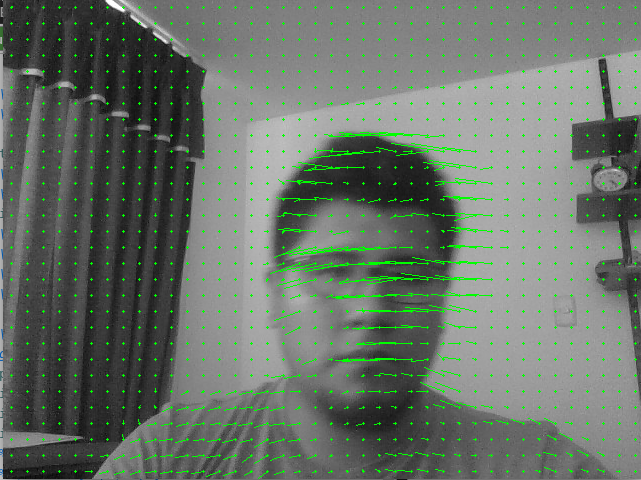
\includegraphics[width=0.4\textwidth]{Kap3/img/Dense_optical_flow_by_lines.png}
  \caption{Dense optical flow by lines}
      \label{fig:Dense_optical_flow_by_lines}
      \end{subfigure}

 % %%\centering
  \caption{Se muestra las 2 técnias de flujo optico.}
  \label{fig:optical-flow2}
\end{figure}




\begin{figure}[h!]

 % \centering
 %\hfill	
  \begin{subfigure}[]{0.4\linewidth}
      \centering
      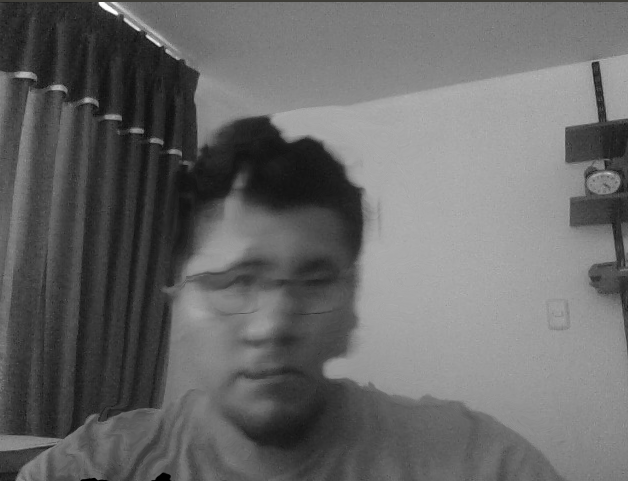
\includegraphics[width=0.4\textwidth]{Kap3/img/Dense_optical_flow_by_warped_image.png}
      \caption{Dense optical flow by warped image}
      \label{fig:Dense_optical_flow_by_warped_image}
  \end{subfigure}
  
   % \centering
  %\hfill	
    \begin{subfigure}[]{0.4\linewidth}
      \centering
      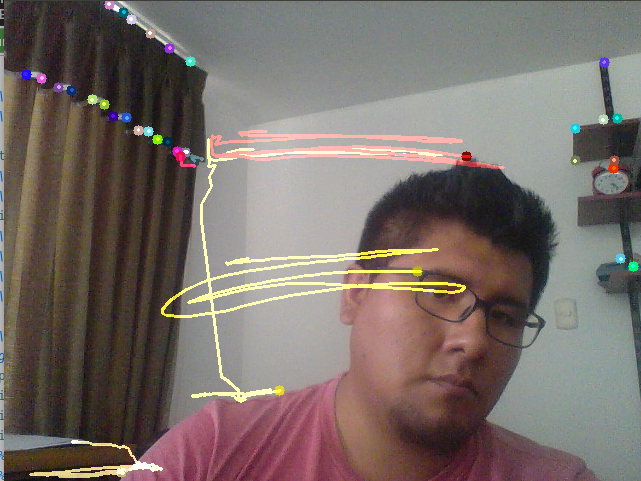
\includegraphics[width=0.4\textwidth]{Kap3/img/Lucas-Kanade_method.png}
      \caption{Lucas-Kanade method}
      \label{fig:Lucas-Kanade_method}
  \end{subfigure}
  
 % %%\centering
  \caption{Se muestra las 2 técnia de lucas kanade para flujo optico.}
  \label{fig:optical-flow1}
\end{figure}



\subsection{Dense Optical Flow}
Lucas-Kanade calcula el flujo óptico para un conjunto de características escasas(Figura \ref{fig:ShiTomasiCorner}). OpenCV proporciona otro algoritmo para encontrar el flujo óptico denso. Calcula el flujo óptico para todos los puntos en el \textit{frame}. Obtenemos una matriz de 2 canales con vectores de flujo óptico,\textbf{ $(u, v)$}. Encontramos su magnitud y dirección. Coloreamos el código para obtener una mejor visualización. La dirección corresponde al valor de tono de la imagen. La magnitud corresponde al plano Valor.(figura \ref{fig:optical-flow1})



\begin{figure}[h!]
\centering
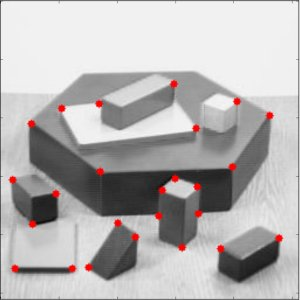
\includegraphics[width=0.6\linewidth]{Kap3/img/shitomasi_block_corner.jpg}
\caption{ en nuestro ejemplo, las esquinas detectadas usando el algoritmo Shi-Tomasi}
\label{fig:ShiTomasiCorner}
\end{figure}


\section{Dataset}

El actual \textit{dataset} \cite{data_set_KTH_baumann2016recognizing} contiene 6 tipos de acciones humanas (\textit{walking, jogging, running, boxing, hand waving y hand clapping}) cada una realizada muchas veces, exactamente por 25 sujetos en 4 diferentes scenarios: (FIGURA \ref{fig:datasetKth} )
\begin{itemize}
\item S1: al aire libre
\item S2: al aire libre con variacion de escala
\item S3: al aire libre con diferente ropa
\item S3: en un ambiente 
\end{itemize}

\begin{figure}[h!]
\centering
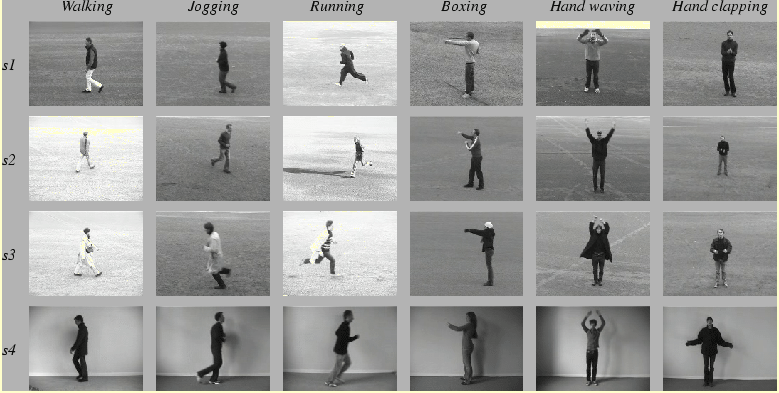
\includegraphics[width=0.6\linewidth]{Kap3/img/datasetKth.png}
\caption{ Se muestra algunos ejemplos de secuencias de un conjunto de datos con seis acciones realizadas por ocho personas diferentes. El conjunto de datos contiene $6*8*4=192$ secuencias y es un subconjunto de una base de datos más grande. Todas las secuencias se obtuvieron con una cámara estacionaria con la velocidad de fotogramas de 25fps y con el submuestreo de la resolución espacial a $160*120$ píxeles.}
\label{fig:datasetKth}
\end{figure}
    
Actualmente el \textit{dataset} contiene un total de 2391 secuencias de imagenes a lo largo de los diferentes videos. Las diferentes secuencias de imagenes fueron tomadas sobre ambientes homogeneos con una camara estatica \textit{"25fps frame rate"}, las secuencias usadas fueron reducidas a una resolucion de 160x120 pixeles y una duracion de 4 por segundo, en promedio.Para nuestros esperimentos reportados sobre \textit{"ICPR'04"} todas la secuencias de video fueron divididas con respecto a:
\begin{itemize}
\item training set (8 personas)
\item validation set (8 personas)
\item test set (9 personas)
\end{itemize}
	
Todas las secuencias de video usan el formato \textit{"AVI"} and estan disponibles (DIVX-compressed version). Hay 25x6x4=600 videos para cada combinación, 25 personas, 6 acciones y 4 escenarios. Cada archivo tiene informacion de las subsecuencias usadas en una secuencia. La subdivision para archivo esta señalado como \textit{"start-frame"} y \textit{"end-frame"} 



\subsection{Convolutional Neural Networks}
El primer trabajo que popularizó Redes Convolucionales en Visión por Computadora fue AlexNet, desarrollado por Alex Krizhevsky, Ilya Sutskever y Geoff Hinton. El AlexNet fue presentado al desafío de ImageNet ILSVRC en 2012 y superó significativamente al segundo subcampeón (error de los 5 primeros del 16\% en comparación con el subcampeón con 26\% de error). La Red tenía una arquitectura muy similar a LeNet, pero era más profunda, más grande y presentaba capas convolucionales apiladas unas encima de otras (anteriormente era común tener sólo una capa de CONV siempre seguida inmediatamente por una capa de POOL). \cite{link10-CS231n_Convolutional_Neural_Networks_for_Visual_Recognition}
